\documentclass[11pt,a4paper]{article}
\usepackage[margin=22mm,headheight=16pt]{geometry}
\usepackage{fontspec,xeCJK}
\setmainfont{Times New Roman}
\setsansfont{Arial}
\setmonofont{Consolas}[Scale=0.86]
\setCJKmainfont{SimSun}[BoldFont=Microsoft YaHei]
\setCJKsansfont{Microsoft YaHei}
\setCJKmonofont{SimSun}
\usepackage{amsmath,amssymb,booktabs,tabularx,array,enumitem}
\usepackage[table]{xcolor}
\usepackage{fancyhdr,fvextra,hyperref,titlesec,graphicx}
\definecolor{inkblue}{HTML}{234D66}
\definecolor{lightblue}{HTML}{EDF3F6}
\definecolor{muted}{HTML}{59636B}
\hypersetup{colorlinks=true,urlcolor=inkblue,linkcolor=inkblue,citecolor=inkblue,
 pdftitle={Feedback-Guided Optimization of Language Models and Programs: Two Small-Scale Case Studies},
 pdfauthor={Research Contributors}}
\setlength{\parindent}{0pt}
\setlength{\parskip}{4pt}
\clubpenalty=10000
\widowpenalty=10000
\displaywidowpenalty=10000
\setlength{\emergencystretch}{2em}
\renewcommand{\baselinestretch}{1.08}
\renewcommand{\arraystretch}{1.15}
\setlist{nosep,leftmargin=1.6em,topsep=3pt}
\setcounter{secnumdepth}{2}
\titleformat{\section}{\Large\bfseries\sffamily\color{inkblue}}{\thesection}{0.6em}{}
\titleformat{\subsection}{\large\bfseries\sffamily\color{inkblue}}{\thesubsection}{0.6em}{}
\titlespacing*{\section}{0pt}{10pt}{6pt}
\titlespacing*{\subsection}{0pt}{8pt}{4pt}
\pagestyle{fancy}
\fancyhf{}
\fancyhead[L]{\footnotesize\sffamily\color{muted} Feedback-guided optimization}
\fancyhead[R]{}
\fancyfoot[C]{\small\color{muted}\thepage}
\renewcommand{\headrulewidth}{0.3pt}
\newcolumntype{Y}{>{\raggedright\arraybackslash}X}
\newcolumntype{P}[1]{>{\raggedright\arraybackslash}p{#1}}
\newcommand{\key}[1]{\textbf{#1}}
\newcommand{\smallheading}[1]{\par\medskip{\large\bfseries\color{inkblue}#1}\par\nobreak\smallskip\nobreak}
\newcommand{\code}[1]{\texttt{#1}}
\newcommand{\tablehead}{\rowcolor{lightblue}}
\newcommand{\figcaption}[2]{\par\begingroup\small\color{muted}\refstepcounter{figure}\label{#1}\textbf{Figure~\thefigure.} #2\par\endgroup\smallskip}
\newcommand{\tabcaption}[2]{\par\smallskip\begingroup\small\refstepcounter{table}\label{#1}\textbf{Table~\thetable.} #2\par\endgroup\smallskip}
\providecommand{\TrainableCount}{Pending}
\providecommand{\TotalCount}{Pending}
\providecommand{\BaseCount}{Pending}
\providecommand{\TrainableRatio}{Pending}
\providecommand{\ReplacedCount}{Pending}




\renewcommand{\TrainableCount}{4,399,104}
\renewcommand{\TotalCount}{498,431,872}
\renewcommand{\BaseCount}{494,032,768}
\renewcommand{\TrainableRatio}{0.8826\%}
\renewcommand{\ReplacedCount}{168}
% Measured constants from the successful A10 BF16 run.
\newcommand{\PPORolloutSteps}{32}
\newcommand{\PPONonzeroBTensors}{168}
\newcommand{\PPOBTensors}{168}
\newcommand{\PPOCriticNonzeroBTensors}{169}
\newcommand{\PPOCriticBTensors}{169}
\newcommand{\PPOBaselineCorrect}{117}
\newcommand{\PPOTrainedCorrect}{122}
\newcommand{\PPOValidationN}{128}
\newcommand{\PPOBaselineAccuracy}{91.40625\%}
\newcommand{\PPOTrainedAccuracy}{95.3125\%}
\newcommand{\PPODelta}{+3.90625}

\let\tablecaption\tabcaption
\begin{document}
\begin{center}
{\LARGE\bfseries\sffamily\color{inkblue} Feedback-Guided Optimization of Language Models and Programs\par}
\vspace{3mm}
{\large Two Small-Scale Empirical Case Studies\par}
\vspace{2mm}
{\small 8 November 2026}
\end{center}
\section*{Abstract}
Feedback can improve either a model's parameters or the program that a model proposes. This study examines both processes through two reproducible, deliberately small experiments. First, a fixed Qwen2.5-0.5B policy was adapted with LoRA and clipped PPO on 512 arithmetic prompts. An NVIDIA A10 BF16 run completed 32 rollout batches, saved Actor and Critic adapters, and successfully reloaded the Actor. On the same 128 development-validation questions, greedy first-line accuracy increased from 117/128 (91.40625\%) to 122/128 (95.3125\%): five corrected answers with no newly incorrect answers. Second, an LLM-guided circle-packing search produced five valid online evaluations from seven saved proposals. Its best online sum of radii was 2.62001380699489; the global winner appeared during initialization rather than a later generation. Independent local execution of that unchanged program produced a valid but numerically different result, 2.6206092130170973, which is retained as a separate measurement. The study distinguishes training diagnostics from paired performance, and online scores from local verification. One seed, development-validation reuse, a manually stopped search and incomplete cost records limit broader conclusions. The main outcome is an inspectable account of feedback, execution and evidence in two optimization workflows.

\section{Introduction}
A scalar reward is useful only when the system can turn it into a controlled change. In policy learning, gradients modify trainable weights; in LLM-guided program search, execution results influence which source-code changes survive. These workflows share a feedback loop, while optimizing different objects with different measurements. Comparing their mechanisms is informative; comparing their raw scores would not be.

The first case studies whether a small language model can complete an adapter-only PPO workflow with a measurable, paired change on a fixed arithmetic task. The second studies how a hosted agent framework generates, evaluates and selects geometric-construction programs. Neither case introduces a new optimization algorithm. Together they provide source-linked experimental records, verified outputs and a practical separation between progress messages and completed outcomes.

\smallheading{Research questions}
\begin{enumerate}[label=\textbf{RQ\arabic*.}]
\item Under a fixed 512-prompt budget, does LoRA-PPO produce a saved, reloadable policy with a higher score on the same 128 arithmetic questions?
\item In a short LLM-guided program search, which candidates improve the measured objective, and what does independent geometric verification establish?
\end{enumerate}

The analysis follows the object that actually changes: adapter matrices in the first case and executable source code in the second. Figure~\ref{fig:feedback} summarizes this distinction. Throughout, numerical results are attributed to their own run, evaluator and execution environment. Historical failures remain available in the evidence package.

\par\noindent\begin{minipage}{\linewidth}
\begin{center}
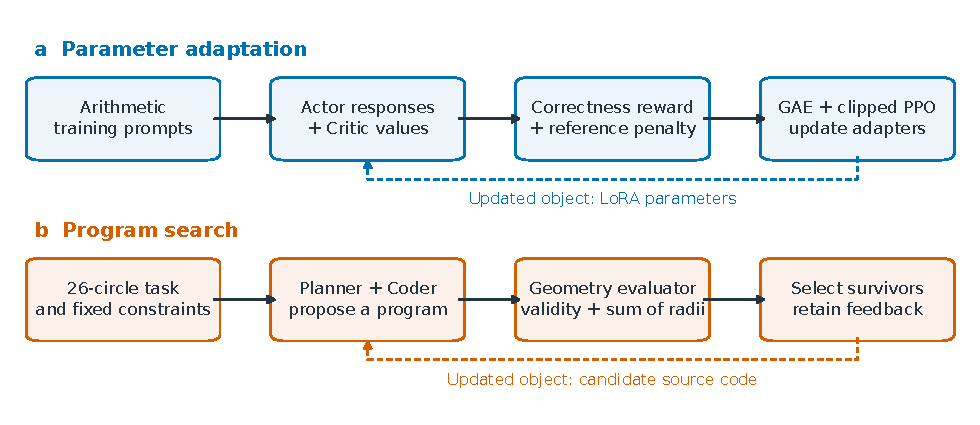
\includegraphics[width=166mm]{../../figures/feedback_mechanisms.pdf}
\end{center}
\figcaption{fig:feedback}{The two feedback mechanisms studied here. Policy optimization changes LoRA parameters through reward and gradient updates; program search changes candidate code through proposal, execution and selection. This is an explanatory mechanism diagram, not a measured comparison of efficiency.}
\end{minipage}\par


\section{Methods and experimental design}
\subsection{Case I: parameter-efficient policy optimization}\label{sec:policy-methods}
\smallheading{Model and trainable representation}
The base model is \path{Qwen/Qwen2.5-0.5B}. Its pinned revision is\newline\code{060db6499f32faf8b98477b0a26969ef7d8b9987}.\cite{qwen} All seven runtime files were verified against the retained manifest, including the original weight SHA-256. ModelScope was the download transport; its \code{master} identifier was not treated as the pinned Hugging Face revision.

LoRA represents a correction to a frozen linear weight with two smaller matrices.\cite{lora,lorasurvey} For positive rank $r$ and column-vector input $\boldsymbol{x}\in\mathbb{R}^{d_{\mathrm{in}}}$,
\[
W\in\mathbb{R}^{d_{\mathrm{out}}\times d_{\mathrm{in}}},\qquad
A\in\mathbb{R}^{r\times d_{\mathrm{in}}},\qquad
B\in\mathbb{R}^{d_{\mathrm{out}}\times r}.
\]
\begin{align}
\Delta W&=\frac{\alpha}{r}BA,\nonumber\\
\boldsymbol{y}&=W\boldsymbol{x}+\boldsymbol{b}
+\frac{\alpha}{r}BA\boldsymbol{x}.\label{eq:lora}
\end{align}
The adapter adds $r(d_{\mathrm{in}}+d_{\mathrm{out}})$ parameters rather than updating all $d_{\mathrm{in}}d_{\mathrm{out}}$ elements of $W$. This is a trainable-parameter comparison, not an estimate of total memory savings: the base model still participates in forward and backward computation.

\par\noindent\begin{minipage}{\linewidth}
\begin{center}
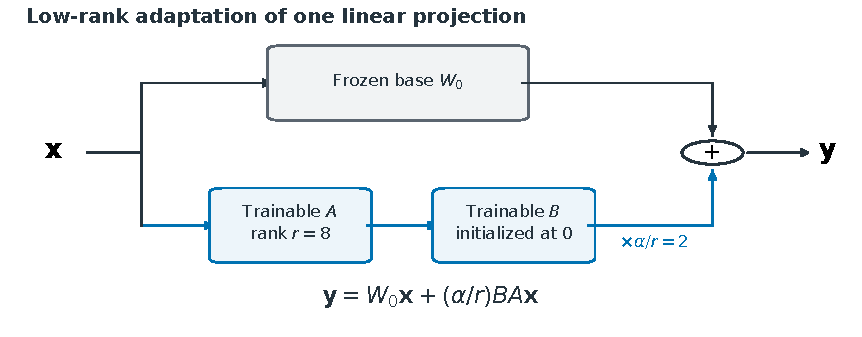
\includegraphics[width=146mm]{../../figures/lora_mechanism.pdf}
\end{center}
\figcaption{fig:lora}{A frozen linear transformation and its low-rank correction. Initializing $B$ to zero preserves the initial output; a nonzero initialization of $A$ permits learning. Inference merging incorporates the correction into $W$ and bypasses the separate branch.}
\end{minipage}\par


For row-batched PyTorch input $X$, Equation~\eqref{eq:lora} becomes
\begin{equation}
Y=XW^{\mathsf T}+\boldsymbol{1}\boldsymbol{b}^{\mathsf T}
+\frac{\alpha}{r}XA^{\mathsf T}B^{\mathsf T}.
\end{equation}
During training, dropout applies only to the adapter input. The equivalence used for merging is evaluated with dropout disabled. Merging performs $W\leftarrow W+\Delta W$ once; an explicit flag prevents adding the correction twice. The manual implementation and its tests are documented in Appendix~\ref{app:implementation}.

\smallheading{Learning rate and batch rationale}
Learning rate sets the scale of an optimizer update. A large value can accelerate initial fitting but destabilize optimization; a smaller value can leave the model under-adapted within a short budget. LoRA's factorized update makes rank, scaling and target modules part of this choice. An empirical analysis reports settings in which LoRA benefits from substantially higher learning rates than full fine-tuning and in which large batches widen the performance gap.\cite{lorablog} Those findings motivate careful tuning, rather than a universal multiplier.

Batch size also changes the number and variability of updates. Without accumulation, 1,024 examples yield 128 updates at batch 8 and 16 at batch 64. A comparison must therefore state whether data volume, update count or compute is held fixed. Here the effective training batch is 8, assembled from microbatches of 1 to limit memory. The Actor/Critic learning rates are $10^{-5}$ and $5\times10^{-5}$. They are fixed starting values; no sweep establishes their optimality.

\smallheading{PPO, value estimation and the reference policy}
OpenRLHF v0.6.0 is fixed to commit \code{bfa85f6fa8cd6214707f93883fac5d08334f4f06}.\cite{openrlhf} The Actor generates responses, the Critic predicts return, and a frozen initial policy provides the reference distribution. A local HTTP reward service grades arithmetic correctness, avoiding a separately trained reward model.

The clipped PPO objective is maximized:\cite{ppo}
\begin{align}
\rho_t(\theta)&=
\frac{\pi_{\theta}(a_t\mid s_t)}{\pi_{\mathrm{old}}(a_t\mid s_t)},\\
J_{\mathrm{clip}}(\theta)&=
\mathbb{E}_t\!\left[
\min\left(\rho_t(\theta)\widehat A_t,\,
\operatorname{clip}(\rho_t(\theta),1-\epsilon,1+\epsilon)\widehat A_t\right)
\right].\label{eq:ppo}
\end{align}
Here $s_t$ is the text prefix, $a_t$ the next token and $\pi_{\mathrm{old}}$ the policy used to collect the rollout. PPO clipping reduces the incentive for an excessive change; it does not strictly bound every update. The implementation minimizes the negative objective, so a signed Actor loss cannot be read as an accuracy measure.

Generalized advantage estimation (GAE) uses the Critic to form
\begin{equation}
\delta_t=\widetilde r_t+\gamma V_\phi(s_{t+1})-V_\phi(s_t),\qquad
\widehat A_t=\sum_{\ell=0}^{T-t-1}(\gamma\lambda)^\ell\delta_{t+\ell},
\end{equation}
with terminal handling supplied by the framework. The shaped reward $\widetilde r_t$ includes the reference-policy KL penalty. This reference differs from the rollout policy in the ratio $\rho_t$: one anchors behavior to the pretrained model, while the other controls an update relative to collected samples.

\par\noindent\begin{minipage}{\linewidth}
\tabcaption{tab:policy-settings}{Fixed settings of the successful policy-learning experiment. A rollout batch is not an optimizer-update count.}
\begin{tabularx}{\linewidth}{@{}P{53mm}Y@{}}
\toprule
\tablehead Setting & Value\\
\midrule
Model / hardware & Qwen2.5-0.5B; one NVIDIA A10; native BF16; ZeRO-2\\
Actor / Critic adapters & $r=8$, $\alpha=16$, dropout $=0$\\
Target projections & q/k/v/o and gate/up/down; Critic also adapts \code{score}\\
Actor / Critic learning rates & $10^{-5}$ / $5\times10^{-5}$; warmup ratio 0.03\\
Rollout / effective train batch & 16 / 8; both microbatches 1\\
PPO / reference regularization & $\epsilon=0.2$; value clip 0.2; initial KL coefficient 0.01\\
GAE / discount & $\lambda=0.95$; $\gamma=1$\\
Training budget & 512 prompts; one episode, one epoch; 32 rollout batches\\
Length / generation & Prompt limit 192; output limit 32 tokens; sampled training responses\\
Seed / memory & Seed 1234; gradient checkpointing\\
\bottomrule
\end{tabularx}
\end{minipage}\par


The budget nominally gives two effective updates per rollout, or 64 per network. Recorded curves use the 32 rollout-batch indices. The Critic includes a LoRA correction on \code{score} because PEFT freezes non-adapter weights; a frozen, unadapted value head would not match the intended configuration.

\smallheading{Data, scoring and paired evaluation}
With seed 1234, the data generator selects 512 training pairs and 128 disjoint validation pairs from $0\le a\le b<50$. Swapped-addend equivalents cannot cross the split. The two examples present in every prompt are excluded from both sets.

Reward is 1 when the first generated line is an integer equal to the sum, and 0 otherwise. Optional sign and horizontal whitespace are allowed; later lines are ignored. The reward service verifies and removes the complete prompt prefix and known padding/end tokens before scoring, preventing prompt examples from earning reward. This metric measures \emph{first-line integer accuracy}; it does not require the model to stop after one answer.

Before and after PPO, the same 128 questions are decoded greedily with a 32-token maximum in BF16. Scores are recomputed from saved responses. An earlier answer-tag rule was revised after observing validation responses, so this split is development validation rather than an untouched final test set.

\subsection{Case II: LLM-guided program search}\label{sec:program-methods}
LLM4AD\_Next, also branded OpenLoopX, searches over executable algorithms.\cite{llm4ad,architecture} An LLM proposes a modification, a Coder implements it within allowed evolution blocks, and a separate Evaluator executes the candidate under fixed constraints. The Orchestrator selects survivors and controls migration and stopping. These roles can share a model; they are not necessarily separately trained agents. Unlike the first case, this search changes program source rather than updating the LLM's weights.

\par\noindent\begin{minipage}{\linewidth}
\begin{center}
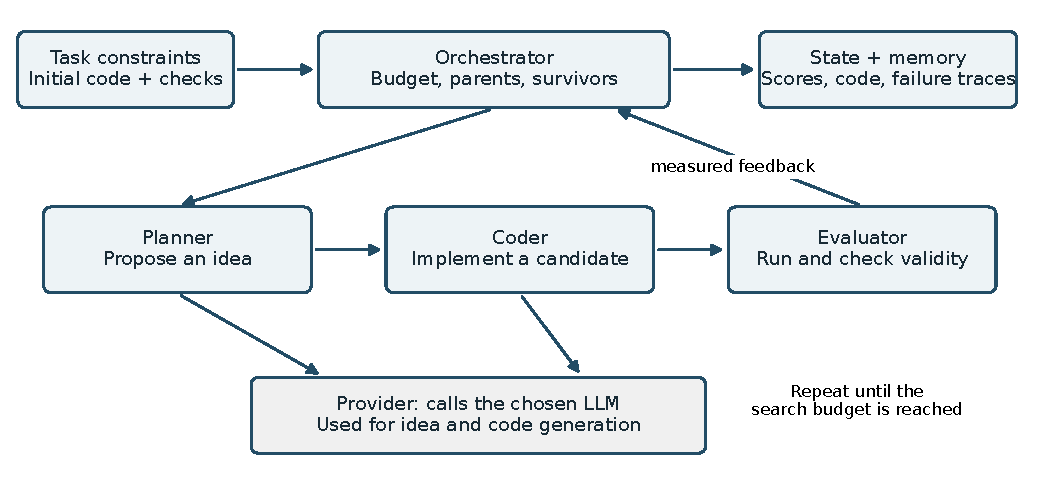
\includegraphics[width=166mm]{../../program_search/figures/framework.pdf}
\end{center}
\figcaption{fig:framework}{The platform's proposal--code--evaluation loop, reconstructed from the pinned architecture and data-flow documentation. The diagram explains component responsibilities and is not a screenshot of an executed task.}
\end{minipage}\par


A complete iteration records the parent program, proposed change, resulting source, score and error information. Island-based search maintains separate populations and periodically exchanges candidates; memory can supply prior solutions or failure explanations.\cite{dataflow,islands,memory} These facilities define possible feedback paths. Their effectiveness must be evaluated from the actual run rather than inferred from their availability.

\smallheading{Objective and fixed geometric constraints}
The selected AlphaEvolve mathematics template requires exactly 26 circles inside the unit square.\cite{benchmark,circle} For center $\boldsymbol c_i=(x_i,y_i)$ and radius $r_i$,
\begin{align}
\max_{\{\boldsymbol c_i,r_i\}_{i=1}^{26}}\quad&
S=\sum_{i=1}^{26}r_i,\label{eq:circle-objective}\\
\text{subject to}\quad&
r_i\ge0,\quad r_i\le x_i\le1-r_i,\quad r_i\le y_i\le1-r_i,\label{eq:circle-boundary}\\
&\|\boldsymbol c_i-\boldsymbol c_j\|_2\ge r_i+r_j\quad(i<j).\label{eq:circle-pairs}
\end{align}
The objective is the sum of radii, not area coverage. The evaluator also requires finite arrays of shapes $(26,2)$ and $(26,)$. Zero-radius circles are permitted. Visual plausibility does not replace these checks.

The official initial constructor was executed locally and accepted by the unchanged geometry-validation method extracted from the evaluator. Its sum was $0.9597642169962063$. This is a preparation measurement, not an online starting score for the later search. The initial geometry and selected program's local reproduction are shown separately from the online trajectory in Section~\ref{sec:program-results}.

\smallheading{Saved search design and observed execution}
The model was \emph{deepseek-v4-flash}, as reported by the platform. The online experiment ran on 31 October 2026. The revised task started at 12:38:01 (UTC+08:00); its final exported workspace was captured at 13:22:05, after which the task was manually stopped.

\par\noindent\begin{minipage}{\linewidth}
\tabcaption{tab:search-settings}{Saved search settings and actual stopping condition. A configured budget is not a count of completed evaluations.}
\begin{tabularx}{\linewidth}{@{}P{58mm}Y@{}}
\toprule
\tablehead Setting & Saved value / actual observation\\
\midrule
Task / seed & 26-circle construction; seed 42\\
Population design & 2 islands; initial target 2 candidates per island\\
Evolution / migration & Target 2 generations; migration interval 1, ring topology\\
Selection & Tournament parent selection; truncation survival\\
Variation & Mutation rate 0.3; crossover rate 0.5; elite ratio 0.2\\
LLM requests & At most 2 concurrent; Coder temperature 0.7\\
Request limits & Coder output ceiling 32,768; saved context limit 8,192\\
Evaluation & Original geometry objective; no evaluator retries\\
Memory & Extraction disabled in saved configuration\\
Actual stopping & Generation 1 completed; generation 2 started; manual stop after export\\
\bottomrule
\end{tabularx}
\end{minipage}\par


The saved YAML records the revised output ceiling (Appendix~\ref{app:platform}). Although memory extraction was disabled, the runtime still logged evaluation-trace embedding. The study does not infer that every memory-related operation was absent. This short demonstration is distinct from the repository's much larger published benchmark.

The explanatory source study uses repository commit \code{dfde353e753e9021fffe88b5b034bf0c84d90b60}. The hosted service may run another revision. Original exports remain in local archival storage; the public subset preserves the candidate and numerical evidence. Local verification uses the unchanged exported geometry method. Local figures retain saved centers and radii with equal axis scaling.

\section{Results}
\subsection{Functional validation before policy learning}
The manual LoRA implementation was exercised with the Qwen model on CPU/float32. It replaced and merged \ReplacedCount{} linear layers: seven targeted projections in each of 24 transformer blocks. The adapters introduced \TrainableCount{} trainable parameters out of \TotalCount{} combined parameters (\TrainableRatio{}). A forward pass and merging completed, and nine lightweight behavior/interface tests passed. These checks establish implementation behavior; the functional entry point contains no language-model optimizer loop. The six implementation responsibilities are summarized in Appendix~\ref{app:implementation}.

\subsection{A saved policy and a paired arithmetic improvement}\label{sec:policy-results}
The independent 16-prompt save/reload check passed before the full A10 experiment. The full run then started from the original base model and completed 512 prompts / \PPORolloutSteps{} batches with exit code 0. All recorded scalars and saved adapter values were finite. Nonzero B tensors were found in all \PPOBTensors{} Actor and \PPOCriticBTensors{} Critic adapter tensors.

The Actor was actually reloaded on the GPU and passed finite forward and generation checks. The Critic adapter passed checksum, finite-value and nonzero-update checks, but was not reloaded. These statements distinguish saved-weight inspection from executable model recovery.

\par\noindent\begin{minipage}{\linewidth}
\tabcaption{tab:paired}{Matched BF16 development-validation outcomes. Both sides use the same 128 questions, greedy decoding, length limit and scoring code.}
\begin{tabularx}{\linewidth}{@{}Y P{39mm}P{39mm}@{}}
\toprule
\tablehead Measurement & Base policy & After PPO\\
\midrule
Correct first-line answers & \PPOBaselineCorrect{}/\PPOValidationN & \PPOTrainedCorrect{}/\PPOValidationN\\
Accuracy & \PPOBaselineAccuracy & \PPOTrainedAccuracy\\
Change & --- & \PPODelta{} percentage points\\
\bottomrule
\end{tabularx}
\end{minipage}\par


\par\noindent\begin{minipage}{\linewidth}
\begin{center}
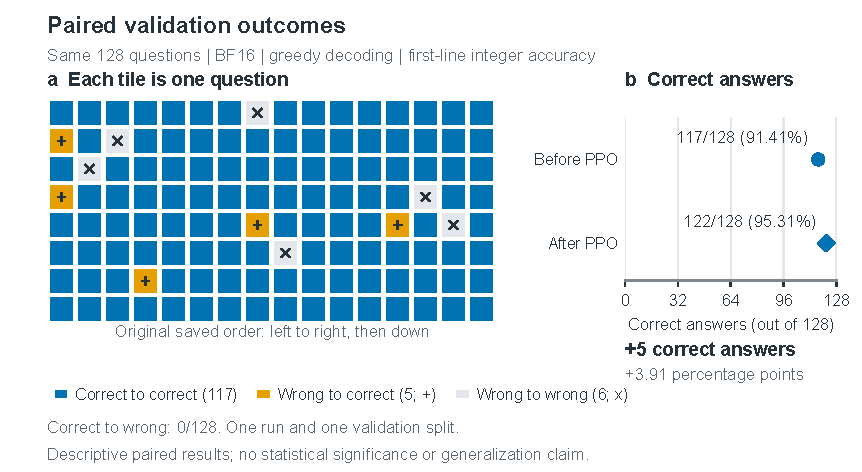
\includegraphics[width=146mm]{../../figures/paired_validation_outcomes.pdf}
\end{center}
\figcaption{fig:paired}{The saved responses are matched question by question. There are 117 correct-to-correct outcomes, five wrong-to-correct outcomes, six wrong-to-wrong outcomes and no correct-to-wrong outcomes. Every outcome is recomputed from the original responses; tiles or marks represent questions rather than repeated experimental runs.}
\end{minipage}\par


The improvement is a net five corrected questions. Examples include $15+23$, changing from 48 to 38, and $45+48$, changing from 133 to 93. Errors remain: $2+33$ changes from 34 to 36, with neither answer correct. This pattern supports a narrow task-level improvement while also showing why a higher aggregate score is not complete arithmetic reliability. The historical T4 baseline of 118/128 uses FP32 and belongs to another run; it is excluded from Table~\ref{tab:paired}.

\subsection{Training dynamics: useful signals with different meanings}
\par\noindent\begin{minipage}{\linewidth}
\begin{center}
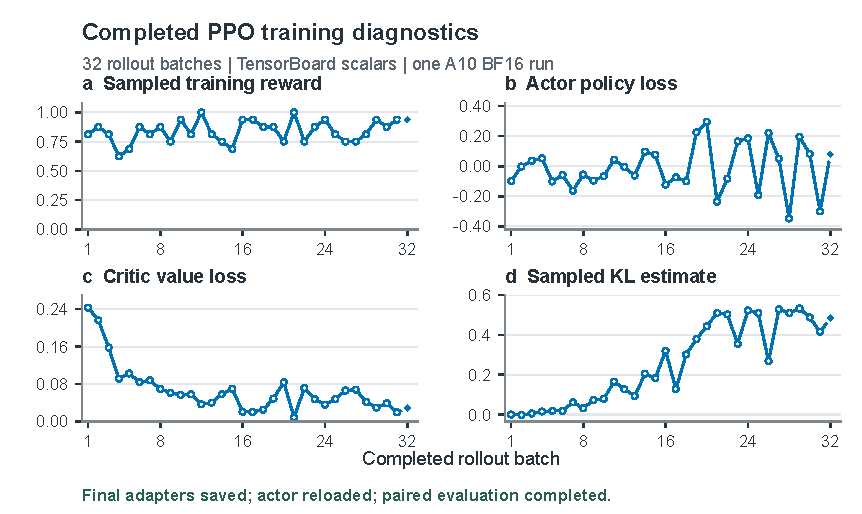
\includegraphics[width=146mm]{../../figures/ppo_training_success.pdf}
\end{center}
\figcaption{fig:ppo-curves}{All 32 measured rollout-batch values of the successful A10 run, without smoothing. Each batch contains 16 prompts. KL is a sampled estimate: its small negative value near the start does not imply a negative theoretical KL divergence.}
\end{minipage}\par


Mean training reward rises from 0.8125 in the first batch to 0.9375 in the last, but ranges between 0.625 and 1.0. Each batch contains different questions and sampled responses, so the endpoints are not a paired estimate of learning. The paired greedy validation in Figure~\ref{fig:paired} provides the direct performance comparison.

Critic loss decreases from approximately 0.2431 to 0.0283, consistent with better fit to the sampled return targets. Actor loss changes sign and fluctuates; it is the signed clipped objective, not a measure of the fraction of correct answers. Estimated KL reaches about 0.485 in the last batch, showing increasing departure from the fixed reference. Neither a lower value loss nor a larger policy departure by itself establishes a task-performance gain.

The logged mean response length changes from 29.125 to 15.5625 tokens between the first and last batches. Some corrected validation responses are shorter, but other answers still continue with additional questions. These observations are compatible with the first-line reward rule; no ablation isolates response length as the cause of improvement.

\smallheading{What the execution evidence adds}
The saved-weight checks close a practical gap left by an earlier run that completed its rollout loop but failed at final serialization. Completion here is established jointly by exit code, full scalar coverage, finite/nonzero adapters, actual Actor reloading and saved paired responses. An isolated progress bar would establish much less. Appendix~\ref{app:recovery} retains both the earlier failure and the later export-manifest ambiguity.

\subsection{Program search: the winner arrived during initialization}\label{sec:program-results}
Seven proposal records are present in the final online export. Five passed the evaluator, one failed implementation with a Python syntax error, and one had no evaluation yet. Only completed valid evaluations enter Table~\ref{tab:online} and Figure~\ref{fig:online}. Generation 0 denotes initialization; island indices are zero-based.

\par\noindent\begin{minipage}{\linewidth}
\tabcaption{tab:online}{Valid online evaluations on 31 October 2026. Times are UTC+08:00; full-precision records remain in the original CSV.}
\begin{tabularx}{\linewidth}{@{}P{28mm}P{13mm}P{14mm}P{30mm}Y@{}}
\toprule
\tablehead Candidate & Gen. & Island & Sum of radii & Time\\
\midrule
\code{fe0aad416d4f} & 0 & 0 & 2.473873492 & 12:46:55\\
\code{4705b8e92e1b} & 0 & 1 & \key{2.620013807} & 13:08:21\\
\code{d3fb7a9f0bab} & 0 & 1 & 2.464972339 & 13:10:19\\
\code{34836c89e4f0} & 1 & 1 & 2.616027976 & 13:18:13\\
\code{a15ea29f0ceb} & 1 & 0 & 2.514353475 & 13:18:47\\
\bottomrule
\end{tabularx}
\end{minipage}\par


\par\noindent\begin{minipage}{\linewidth}
\begin{center}
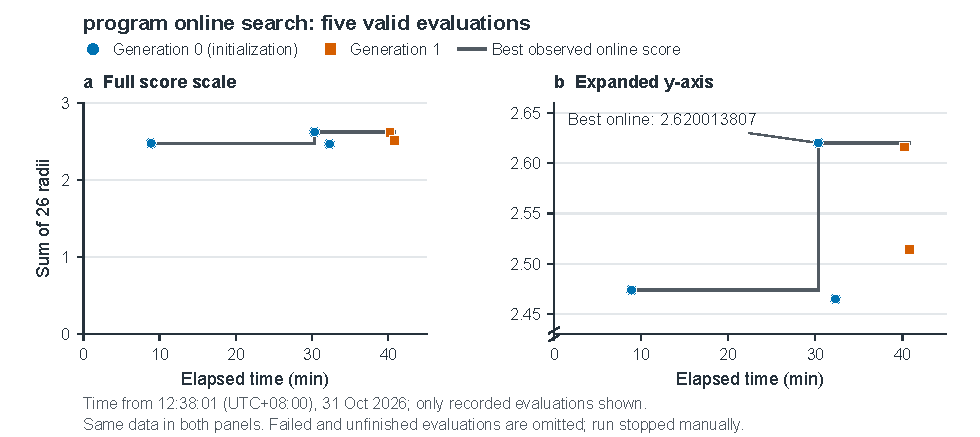
\includegraphics[width=166mm]{../../program_search/figures/online_progress.pdf}
\end{center}
\figcaption{fig:online}{The same five online scores at full scale and with an explicitly expanded y-axis. Circles denote initialization and squares generation 1; the step line is the running best. Failed or missing evaluations are not plotted as zero, and the line is not extended beyond observed evaluations.}
\end{minipage}\par


For valid candidates observed by time $t$, the incumbent is
\begin{equation}
S_t^\star=\max_{a\in\mathcal V_t}S(a),\qquad\mathcal V_t\ne\varnothing.
\end{equation}
The best online score is 2.62001380699489, from initial candidate \code{4705b8e92e1b}. A generation-1 child improves its own parent from 2.473873492 to 2.514353475, but neither observed child beats the global incumbent. Local parent improvement and improvement of the overall search are therefore different events. The run demonstrates generation, execution and selection; its short, manually stopped trajectory establishes neither convergence nor an optimum.

\subsection{Independent geometry: a separate result, not a replacement score}
The selected program tries eight deterministic starting layouts and uses SLSQP to adjust centers and radii jointly. With centers fixed, its radius allocation is a linear program:
\begin{equation}
\max_{\boldsymbol r}\sum_i r_i\quad\text{subject to}\quad
0\le r_i\le b_i,\quad r_i+r_j\le d_{ij}\quad(i<j),
\end{equation}
where $b_i=\min(x_i,y_i,1-x_i,1-y_i)$ and $d_{ij}=\|\boldsymbol c_i-\boldsymbol c_j\|_2$. A final conservative radius repair reduces numerical violations. Optimal radii for fixed centers do not establish a globally optimal layout.

\par\noindent\begin{minipage}{\linewidth}
\begin{center}
\begin{minipage}[t]{0.47\linewidth}\centering
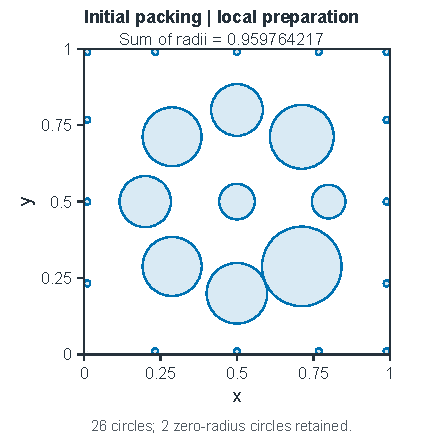
\includegraphics[width=75mm]{../../program_search/figures/initial_packing.pdf}\\
{\small (a) Official initial constructor}
\end{minipage}\hfill
\begin{minipage}[t]{0.47\linewidth}\centering
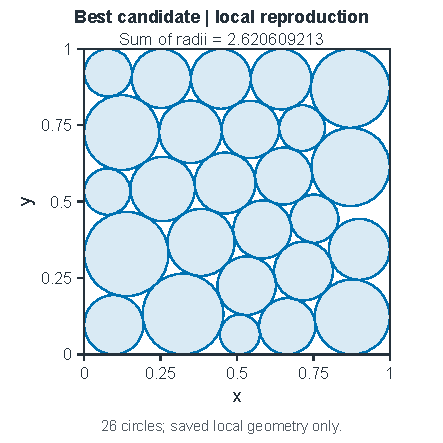
\includegraphics[width=75mm]{../../program_search/figures/online_best_reproduced.pdf}\\
{\small (b) Selected program, re-executed locally}
\end{minipage}
\end{center}
\figcaption{fig:geometry}{Two separate local geometry records. Panel (a) has sum 0.9597642169962063; panel (b) has sum 2.6206092130170973. The plots preserve the original saved centers, radii and equal scale. Panel (b) is not the server's original geometry and does not replace its online score.}
\end{minipage}\par


Unmodified local execution of the selected source took about 4.76 seconds using Python 3.14.2, NumPy 2.4.4 and SciPy 1.17.1. The original geometry method accepted all 26 circles. Minimum boundary and pair gaps were approximately $1.38\times10^{-12}$ and $1.02\times10^{-12}$: positive in the saved calculation, but numerically small.

The local sum, 2.6206092130170973, exceeds the online record by approximately 0.000595406. Runtime or numerical differences are plausible explanations; their cause was not isolated. The online experiment result remains 2.62001380699489. Likewise, the local initial-constructor value is not a same-run online baseline, so no online percentage gain is computed from it.

\section{Discussion}
\subsection{What feedback accomplished in the two cases}
In policy learning, the updated object is a set of adapter matrices, and the decisive evidence is the saved policy's paired behavior. Here five previously incorrect questions became correct while 117 remained correct. Training reward and loss help describe optimization, but they cannot substitute for that comparison.

In program search, the updated object is executable code. Candidate validity is a prerequisite for interpreting its score, and retaining a strong incumbent matters even when a later child improves only its own parent. The global winner's appearance during initialization is an informative result: the observed trajectory provides no evidence that subsequent evolution improved the best solution.

These cases share an evaluator-mediated feedback cycle, but not a common outcome scale. A language-model accuracy difference and a geometric radius sum are not combined into a single performance claim. Independent verification instead asks a common question: can the stated outcome be traced to a valid saved artifact under a specified evaluation procedure?

\subsection{Limitations and alternative explanations}
\begin{itemize}
\item \key{One seed and a narrow task.} The policy experiment uses one seed, a 0.5B model and a short addition task. There is no learning-rate, batch-size or rank ablation, no repeated-run uncertainty estimate and no evidence of broader reasoning gains.
\item \key{Development validation.} The first-line protocol was revised after inspecting validation responses. Although the final before/after questions and settings match, this is not an untouched test set. Extra text after the first answer line is not penalized.
\item \key{Implementation and precision.} PPO explicitly uses eager attention; the unchanged paired evaluator may select SDPA. Both evaluations use BF16 on the same A10. The older FP32 T4 result is a separate record, not the baseline for the successful run.
\item \key{Saved Critic state.} Actor reloading was verified. The Critic export contains LoRA matrices but omits the underlying randomly initialized value-head weight. These files alone cannot reconstruct the full trained value function; neither independent Critic recovery nor complete optimizer-state recovery is established.
\item \key{Short program-search coverage.} Five valid evaluations cannot characterize the search distribution. The configured budget was not automatically completed, and no score is assigned to an unfinished evaluation.
\item \key{Numerical and service reproducibility.} The local and online circle scores differ slightly. Versioned source does not guarantee identical remote LLM responses, hosted revisions or numerical trajectories. Total task cost and credits are unavailable.
\end{itemize}

\subsection{Engineering experience as part of the evidence}
The main practical challenge was making each stage observable and preservable. Earlier GPU availability and network failures repeatedly blocked dependency installation. A prior PPO loop completed but failed a tied-weight serialization check. The successful continuation therefore required a real CUDA/optimizer preflight, a short independent save/reload check and a fresh full run with protected outputs.

The final environment retains a visible exception: upstream OpenRLHF declares FlashAttention, which is absent. Source-hash-checked delayed imports restrict execution to the supported single-GPU eager path; they do not replace FlashAttention's computation or permit ring attention. The base model, PPO calculations, data and budget remain unchanged. This experience supports a methodological lesson: diagnose the failing stage and verify the resulting artifact, rather than treating elapsed time or a completed loop as experimental completion. Detailed provenance and the repeated-start guard are recorded in Appendix~\ref{app:recovery}.

\section{Future work: two testable improvements to program search}\label{sec:future}
\subsection{Evidence-grounded reflection and selective memory}
The framework already offers reflection and scoped memory.\cite{memory} A useful extension would store verified repair lessons linked to candidate and evaluator versions. Failures would identify specific overlapping circles, boundary violations, array-shape errors or timeouts, with the relevant code. Retrieval would favor a few task-relevant, nonduplicate lessons and distinguish tested repairs from unverified suggestions.

The hypothesis is that more precise feedback reduces repeated invalid programs. Reflection and retrieval also consume tokens and can preserve stale assumptions. A controlled study should compare otherwise identical runs with and without evidence-grounded memory under the same model, evaluator and call budget across several seeds. Primary measurements would be valid-candidate rate, repeated failure rate, best valid score and cost per valid improvement.

\subsection{Diverse proposals with adaptive effort allocation}
Island search and migration already exist in the framework.\cite{islands} A further policy could reserve distinct roles for local refinement, alternative spatial arrangements and constraint-robust construction. Exact duplicate programs could be rejected before another full evaluation, while a reserved exploration budget would prevent all effort from following the current winner. Allocation would respond to measured valid improvements rather than the novelty of an explanation.

The hypothesis is that distinct directions and adaptive allocation improve search efficiency. They can also waste a short budget on weak directions. Compare fixed, uniform prompting and allocation with role-diverse, adaptive allocation at equal total LLM-call or token cost. Across multiple seeds, report median best valid score and spread, unique valid candidates and time to a predeclared target. Keep the evaluator outside editable program blocks and independently verify every saved winner. Neither proposal was experimentally compared in this study.

\section{Conclusion}
A complete A10 LoRA-PPO experiment produced saved adapters, a reloadable Actor and a paired increase from 117 to 122 correct arithmetic answers out of 128. A separate LLM-guided program search produced five valid evaluations and an online best radius sum of 2.62001380699489; independent local geometry verification remained a distinct measurement. The two cases show how feedback operates on different artifacts and why execution, selection and validation records are essential to a reproducible empirical claim. Their small scale supports these specific observations, not a general ranking of methods.

\begin{thebibliography}{99}
\small
\setlength{\itemsep}{4pt}
\bibitem{lora}
E. J. Hu et al. \textit{LoRA: Low-Rank Adaptation of Large Language Models}. 2021.
\href{https://arxiv.org/abs/2106.09685}{arXiv:2106.09685}.
\bibitem{lorasurvey}
Y. Mao et al. \textit{A Survey on LoRA of Large Language Models}. 2024.
\href{https://arxiv.org/abs/2407.11046}{arXiv:2407.11046}.
\bibitem{lorablog}
J. Schulman et al. \textit{LoRA Without Regret}. Thinking Machines Lab, 29 September 2025.
\href{https://thinkingmachines.ai/blog/lora/}{Empirical analysis of LoRA fine-tuning}.
\bibitem{qwen}
Qwen Team. \href{https://huggingface.co/Qwen/Qwen2.5-0.5B}{Qwen2.5-0.5B model card};
\href{https://modelscope.cn/models/Qwen/Qwen2.5-0.5B}{official ModelScope repository}.
Pinned Hugging Face revision: \code{060db6499f32faf8b98477b0a26969ef7d8b9987}.
\bibitem{ppo}
J. Schulman, F. Wolski, P. Dhariwal, A. Radford and O. Klimov.
\textit{Proximal Policy Optimization Algorithms}. 2017.
\href{https://arxiv.org/abs/1707.06347}{arXiv:1707.06347}.
\bibitem{openrlhf}
OpenRLHF Team. OpenRLHF v0.6.0, commit \code{bfa85f6fa8cd6214707f93883fac5d08334f4f06}.
\href{https://github.com/OpenRLHF/OpenRLHF/blob/bfa85f6fa8cd6214707f93883fac5d08334f4f06/openrlhf/cli/train_ppo.py}{Training entry point};
\href{https://github.com/OpenRLHF/OpenRLHF/blob/bfa85f6fa8cd6214707f93883fac5d08334f4f06/openrlhf/models/actor.py}{Actor};
\href{https://github.com/OpenRLHF/OpenRLHF/blob/bfa85f6fa8cd6214707f93883fac5d08334f4f06/openrlhf/models/model.py}{Critic};
\href{https://github.com/OpenRLHF/OpenRLHF/blob/bfa85f6fa8cd6214707f93883fac5d08334f4f06/openrlhf/trainer/ppo_utils/experience_maker.py}{sampling and advantage estimation};
\href{https://github.com/OpenRLHF/OpenRLHF/blob/bfa85f6fa8cd6214707f93883fac5d08334f4f06/openrlhf/utils/deepspeed/deepspeed.py}{saving logic}.
\bibitem{torch}
PyTorch Team. PyTorch v2.5.1.
\href{https://github.com/pytorch/pytorch/blob/v2.5.1/torch/cuda/__init__.py}{CUDA BF16 capability detection and the \code{including\_emulation} argument}.
\bibitem{llm4ad}
Optima-CityU. \href{https://github.com/Optima-CityU/LLM4AD_Next/tree/dfde353e753e9021fffe88b5b034bf0c84d90b60}{LLM4AD\_Next / OpenLoopX};
\href{https://llm4ad-next.cn/}{hosted service}.
Source-study commit: \code{dfde353e753e9021fffe88b5b034bf0c84d90b60}.
\bibitem{architecture}
LLM4AD\_Next. \href{https://github.com/Optima-CityU/LLM4AD_Next/blob/dfde353e753e9021fffe88b5b034bf0c84d90b60/docs/en/architecture/overview.md}{Architecture Overview}.
Pinned source revision as above.
\bibitem{dataflow}
LLM4AD\_Next. \href{https://github.com/Optima-CityU/LLM4AD_Next/blob/dfde353e753e9021fffe88b5b034bf0c84d90b60/docs/en/architecture/data-flow.md}{Data Flow}.
Initialization, evolution, state and export boundaries.
\bibitem{islands}
LLM4AD\_Next. \href{https://github.com/Optima-CityU/LLM4AD_Next/blob/dfde353e753e9021fffe88b5b034bf0c84d90b60/docs/en/guides/island-ga.md}{Island GA guide}.
\bibitem{memory}
LLM4AD\_Next. \href{https://github.com/Optima-CityU/LLM4AD_Next/blob/dfde353e753e9021fffe88b5b034bf0c84d90b60/docs/en/guides/memory.md}{Long-term Memory guide}.
\bibitem{benchmark}
LLM4AD\_Next. \href{https://github.com/Optima-CityU/LLM4AD_Next/blob/dfde353e753e9021fffe88b5b034bf0c84d90b60/examples/applications/alphaevolve_math_benchmark/README.md}{AlphaEvolve Mathematics Benchmark Suite}.
Task definitions, objective directions and published-score provenance.
\bibitem{circle}
LLM4AD\_Next circle-packing example:
\href{https://github.com/Optima-CityU/LLM4AD_Next/blob/dfde353e753e9021fffe88b5b034bf0c84d90b60/examples/applications/alphaevolve_math_benchmark/circle_packing/code_config.yaml}{configuration};
\href{https://github.com/Optima-CityU/LLM4AD_Next/blob/dfde353e753e9021fffe88b5b034bf0c84d90b60/examples/applications/alphaevolve_math_benchmark/circle_packing/algorithm/solve.py}{initial constructor};
\href{https://github.com/Optima-CityU/LLM4AD_Next/blob/dfde353e753e9021fffe88b5b034bf0c84d90b60/examples/applications/alphaevolve_math_benchmark/circle_packing/evaluator.py}{geometry evaluator}.
\bibitem{deepseek}
DeepSeek. \href{https://api-docs.deepseek.com/guides/thinking_mode/}{Thinking Mode};
\href{https://api-docs.deepseek.com/api/create-chat-completion/}{Chat Completions API}.
\end{thebibliography}


\clearpage
\appendix
\section{Implementation checks}\label{app:implementation}
The manual module \path{policy_adaptation/lora_training.py} implements argument validation, shared frozen base weights, Kaiming-uniform initialization of $A$, zero initialization of $B$, the scaled adapter branch, idempotent merging, nested module injection and trainable-parameter counting. The functional model check used CPU/float32 and replaced 168 projections in the 24-layer Qwen model. It reported 494,032,768 base parameters and 4,399,104 adapter parameters, or 0.8826\% of the combined model. Its forward pass and merging are functional checks, not a language-model optimizer loop.

Nine lightweight tests covered initial equality, weight sharing, a nonzero adapter formula, output-preserving and idempotent merging, frozen-base optimizer updates, nested injection/counting, invalid inputs, disjoint arithmetic data and response-only rewards with real local HTTP requests. The functional configuration used $r=8$, $\alpha=16$ and dropout 0.05; PPO used dropout 0.

\section{Search record and reproducibility boundary}\label{app:platform}
The hosted run's revised configuration started at 12:38:01 on 31 October 2026 (UTC+08:00). Its last retained event was at 13:21:18.838, and the final workspace was exported at 13:22:05. The task was then manually stopped; no automatic completion event is claimed. Five valid evaluations from seven saved proposals define the online result.

An earlier attempt produced five proposals without a valid evaluation; four completed code replies were empty. The revised run raised the output ceiling from 4,096 to 32,768 and reduced the search budget. Multiple changes and incomplete request finish reasons prevent a causal claim about which change resolved that failure. The preserved Planner records contain 70,376 tokens; this is not a complete task-cost estimate.

The source study pins LLM4AD\_Next to \code{dfde353e753e9021fffe88b5b034bf0c84d90b60}; the hosted service may use another revision. Candidate source, five evaluation records, saved configuration and independently checked geometry are published without account-specific interface captures. The actual server geometry of the online winner was not exported; the plotted winning geometry is a separate local re-execution.

\section{Historical serialization failure and successful recovery}\label{app:recovery}
An earlier FP32 T4 run completed 512 prompts / 32 rollout batches but failed at final serialization with a missing tied output-head alias:
\begin{Verbatim}[fontsize=\small,breaklines=true,frame=single]
AssertionError: mismatch keys {'base_model.model.lm_head.weight'}
RuntimeError: training failed (exit 1)
\end{Verbatim}
Its development baseline was 118/128; it has no valid final adapter or post-training validation. That baseline is not paired with the later A10 result. The preserved rounded scalar table describes that historical loop only.

\begin{center}
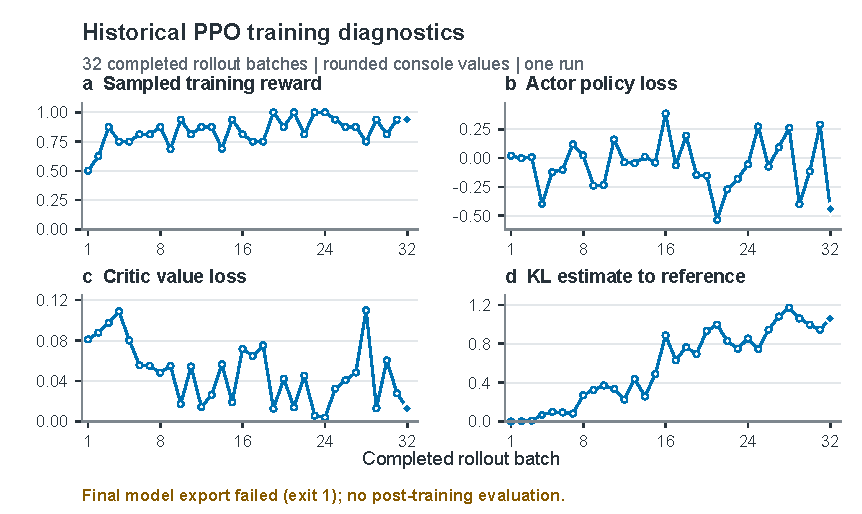
\includegraphics[width=146mm]{../../figures/observed_attempt.pdf}
\end{center}
\figcaption{fig:historical}{Historical T4 diagnostics at displayed console precision. The final-save failure occurred after these batches; the curves are neither the successful A10 run nor post-training validation.}

The save repair accepts a missing output-head name only when it aliases the exact same Parameter as the input embedding; a genuinely missing independent weight remains an error. A separate sampler repair supplies the missing \code{pad\_len=None}. The single-GPU eager route delays only unused ring-operation imports, with source hashes checked. Ring attention and packing remain disabled, and invoking that ring operation still requires FlashAttention. The declared package exception is retained: OpenRLHF 0.6.0 requires FlashAttention, which is absent. Real CUDA Actor/Critic forward/backward and FusedAdam-update checks passed before the independent 16-prompt save/reload check and fresh full run.

The successful environment used Python 3.10, PyTorch 2.5.1+cu124, Transformers 4.48.3, PEFT 0.14.0, DeepSpeed 0.16.3 and Ray 2.42.0. The evaluator may use SDPA; PPO explicitly used eager attention. The complete run finished at 09:48:14 UTC on 8 November 2026. A second invocation nine seconds later was refused by the existing-output guard. Its export manifest reports failure for that later invocation; it does not invalidate the prior successful exit, 32-batch metrics, saved finite/nonzero adapters, actual Actor reload and paired responses. Original local exports are preserved separately from the portable public evidence subset. Critic reloading and complete PPO optimizer-state recovery were not performed.

\section{Reading and reproducing the evidence}
\path{policy_adaptation/} contains the manual adapter, fixed training launcher, evaluator, reward service and compatibility repairs. Its \path{results/} records the A10 paired responses, scalar metrics and saved adapters. The historical T4 table remains separate. \path{program_search/} contains the exported best constructor, original geometry checks, saved online evaluations and independent local geometry. Plotting scripts read these saved records and do not repeat training or online search. Public copies normalize identity-bearing or machine-specific paths; this changes neither numerical results nor adapter tensors.

The fresh-environment setup recipe has not itself been validated through another complete GPU experiment. Hosted model availability, network access and GPU allocation remain external conditions. Consult the repository README for installation groups, basic checks and explicit training commands. Running a lightweight test, a plotting script or local geometry optimization is not a new PPO experiment or hosted search.

\end{document}
